
\section{Study2: Structuring, Source Management, and Larger Deployment}

Study 2 aims to incorporating findings from Study 1 to further develop the prototype system to support the next steps in exploratory search tasks --- managing the multiple opened sources during foraging and structuring the collected information. I also plan to further refine the current implementation to a stable state in order to conduct a larger field deployment in order to investigate the costs and benefits of longer term usage and in more realistic scenarios. Preliminary tests for Study 1 already revealed a few user needs that were out of the scope of Study 1 but can be further explored with Study 2:

\begin{enumerate}[label=\alph*)]
    \item The focus of Study 1 is to explore using entities mentioned across webpages as a backbone structure to support gathering information across multiple webpages, but participants also express the need for creating more flexible structures, cited their current practices of using word processors (such as Google Docs) to create outlines or tables to structure both information copied from webpages and manual notes about their own thoughts. One potential direction is to extend the current prototype to support such structures and investigate ways to support structuring across multiple webpages. For example, automatically focus on a relevant part of a user-created outline when reading an individual webpage based on text similarity instead of just relying on common entity mentions. 
    \item We also observed that exploratory searches can lead to large numbers of open tabs that were difficult to manage for the users. These tabs can be overloaded with different purposes, such as to-do tasks, reminders for things to go back to, or potential future references. Popular bookmarking browser extensions such as OneTab\footnote{\url{https://www.one-tab.com/}} allow users to save and re-open sets of tabs as bookmarks for archiving and resumption, but at the same time takes away many features of browser tabs such as reminding.
    I plan to conduct interviews to better understand how people utilize browser tabs when during productivity tasks, and potentially use the findings to further develop features for saving and managing webpages while foraging and structuring from a large number of webpages. 
\end{enumerate}

Note that this is a tentative list that is subject to change based on findings from Study 1 and early user study, but the goal here is to identify a small and crucial set of important features that have a high impact on public adoption while maintaining the scope of the thesis. 
In the current prototype design, users can create note cards by typing or capturing parts of a webpage, and organize their cards into an outline structure (Figure \ref{fig:screenshot}). Findings from study 1 that focused on connecting different webpages could inform the further development of the current system to support tightly integrating foraging and structuring by connecting information on the webpages to the user-created outline structures.

%\begin{figure}
% \centering
% 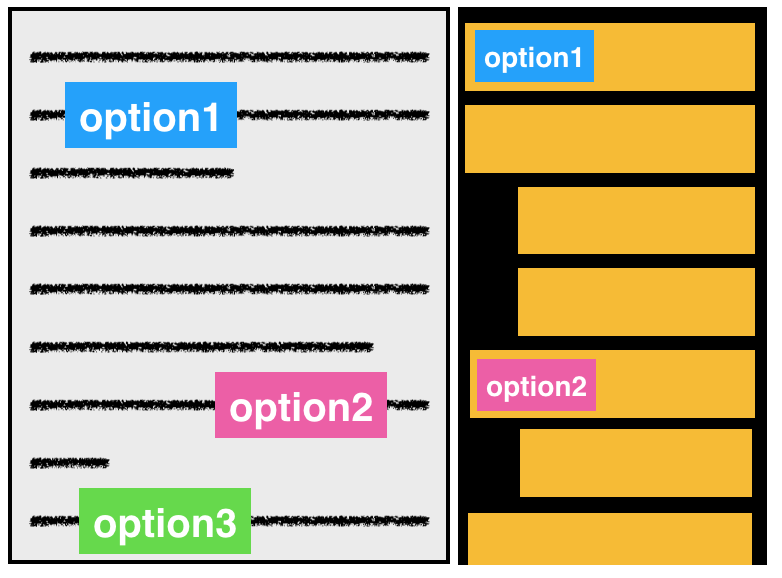
\includegraphics[width=0.31\textwidth]{images/outline.p%ng}
% \caption{The second study plans to incorporate findings %from the first study to build a browser extension that can %better support foraging and structuring across multiple %%webpages.}
% \label{fig:outline}
%\%end{figure}

\begin{figure}
    \centering
    \frame{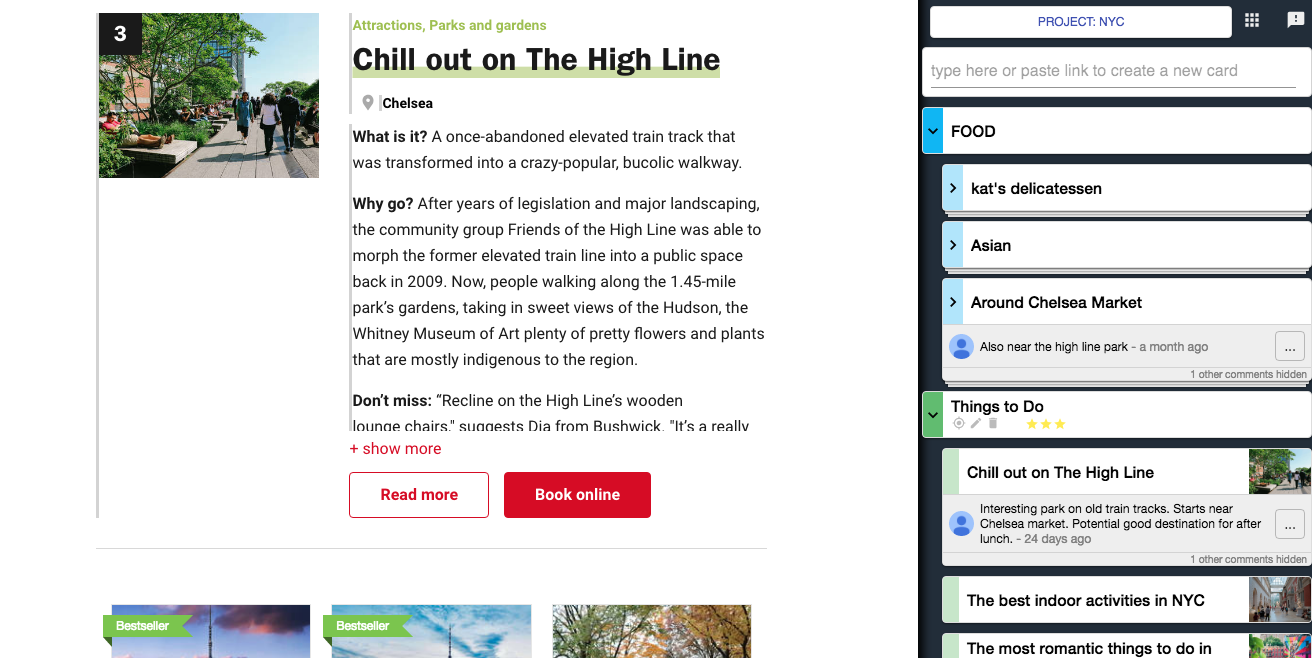
\includegraphics[width=1.0\textwidth]{images/screenshot2.png}}
    \caption{Current design of a prototype system for capturing and structuring findings into outlines during exploratory search. In study 2, I plan to augment the system with findings from study 1 and enable entity support using the gather and propagate mechanisms.}
    \label{fig:screenshot}
\end{figure}